\documentclass[twocolumn,11pt]{article}
\setlength{\textheight}{9truein}
\setlength{\topmargin}{-0.9truein}
\setlength{\parindent}{0pt}
\setlength{\parskip}{10pt}
\setlength{\columnsep}{.4in}

\usepackage{amsmath,amsfonts,amssymb,amsthm,bm,caption,calc,ifthen,graphicx,url,hyperref}

\begin{document}
\pagestyle{plain}
\onecolumn
ASTP720 
\newline Homework 7
\newline Will Wainwright
\newline Repository: \href{https://github.com/wjwainwright/ASTP720}{https://github.com/wjwainwright/ASTP720}

\section*{Discussion}
Given the time crunch of getting all these assignments done on time, I had to use numpy's FFT method to save time. I created the frequency array using the Nyquist frequency as the cutoff. I constructed a plot of the power spectrum vs frequency, and found the position of the spike in the signal. The frequency at which this spike occurred was $0.00220375Hz$, with a strain of $6.328826094262944e-22$. This gives the system a mass of $1.3869277048001234 M_\odot$ and a separation of $0.6585315503485444 R_\odot$. This is consistent with the theoretical mass limit of a white dwarf being $1.44 M_\odot$. Given more time, I would certainly have taken a crack at writing my own FFT algorithm.


\begin{figure}[!h]
	\centering
	\noindent
	\makebox[\textwidth]{
      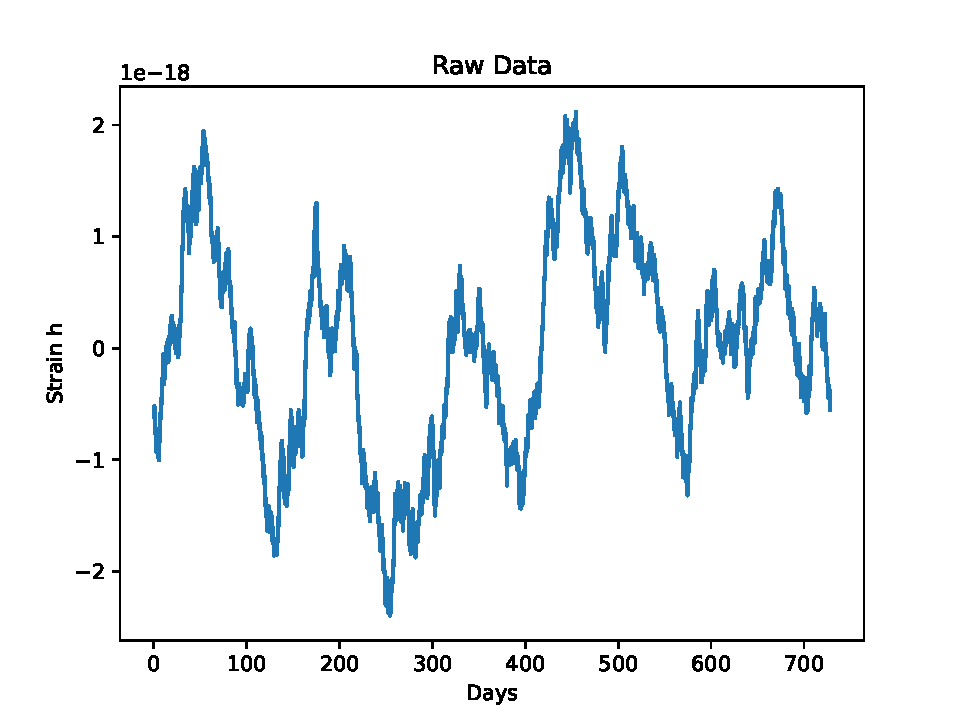
\includegraphics[width=4.5in]{strain.pdf}}
      \caption{Plot of the strain data over the 2 year period.}
\end{figure}

\begin{figure}[!h]
	\centering
	\noindent
	\makebox[\textwidth]{
      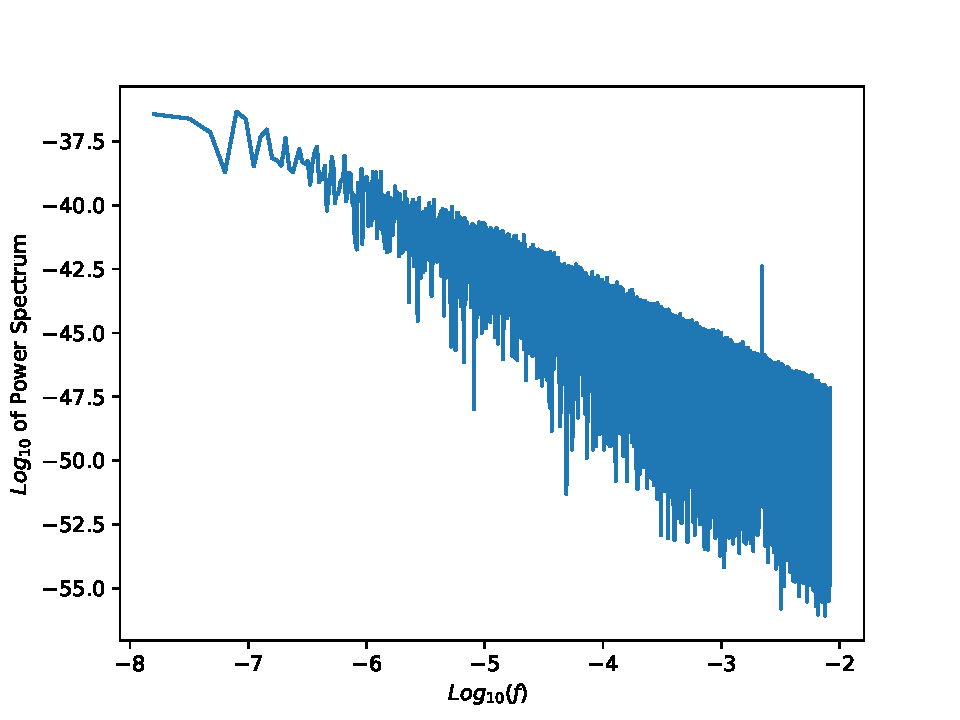
\includegraphics[width=4.5in]{fft.pdf}}
      \caption{Plot of power spectrum of the FFT. Normalized by dividing by N data points and multiplying by 2.}
\end{figure}




\end{document}